\documentclass[11pt,a4paper]{article}
\usepackage[margin=2.5cm]{geometry}
\usepackage{amsmath,amssymb,booktabs,graphicx,xcolor,hyperref,microtype}
\usepackage{authblk}
\hypersetup{colorlinks=true,linkcolor=blue,citecolor=blue,urlcolor=blue}

\title{\textbf{Paper 60: Causal Purity as an Independent Control Parameter\\
in an Ising Spin System}\\
\large Cross-Substrate Verification of the Causal-Purity Universality Class}

\author[1]{Gabriel Aubin-Moreau}
\affil[1]{Independent research}
\date{March 2026}

\begin{document}
\maketitle

\begin{abstract}
Papers~57--59 established that causal purity $P_\mathrm{causal}$ controls a new
type of non-equilibrium order in VCML --- distinct from temperature-driven phase
transitions.
The universality class claim requires the same mechanism to appear in a different
physical substrate.

We test this in a 2D Ising spin system augmented with a VCSM-lite memory layer
(slow field $\phi$, updated by zone-attributed wave events, gated by causal purity).
The Ising model has one standard order parameter (magnetisation $m$, controlled
by temperature $T$); the VCSM layer adds a second order parameter
($S_\phi = |\bar\phi_{\rm zone0} - \bar\phi_{\rm zone1}|/\sigma_\phi$,
controlled by $P_\mathrm{causal}$).

\textbf{Key result:} $m$ depends only on $T$
(columns of the $(T, P_\mathrm{causal})$ phase diagram are constant).
$S_\phi$ depends monotonically on $P_\mathrm{causal}$ at \emph{all}
temperatures, including $T > T_c$ where spins are completely disordered
($m = 0.07$, $S_\phi$ ranges from $0.51$ to $0.91$).

The two order parameters are \textbf{orthogonal control parameters}:
temperature controls spin order; causal purity controls memory order.
The memory layer develops zone-specific structure even when the
underlying spin substrate is thermally disordered --- exactly the
condition under which attractor persistence (ferromagnet-like)
fails and reconstructive persistence (VCSM-like) is the only available mechanism.

This is the first cross-substrate demonstration that causal purity is an
independent control parameter for non-equilibrium order.
It supports the universality class hypothesis: VCSM describes a new class
of purity-controlled stochastic field dynamics, not specific to VCML.
\end{abstract}

%──────────────────────────────────────────────────────────────────────────────
\section{Introduction and Motivation}

Paper~59 derived the Model~A field equation for VCML's fieldM:
\begin{equation}
  \partial_t\phi = -\kappa\phi + D\nabla^2\phi + r_w FA\,s(x) + \eta,
  \quad
  \langle\eta^2\rangle \propto (1-P_\mathrm{sp})^2 V_\mathrm{bnd}
  + (1-P_\mathrm{temp})^2 V_\mathrm{temp}.
\end{equation}
The noise amplitude is controlled by \emph{causal purity}, not temperature.
Most field theories use temperature as the noise control parameter;
in VCML, causal purity plays that role.

For this to be a genuine universality class,
the same purity-controlled phase transition must appear in different
physical substrates.
The simplest clean test: a 2D Ising ferromagnet (the prototype attractor
persistence system) with a VCSM-lite memory layer on top.

If $S_\phi$ transitions with $P_\mathrm{causal}$ while $m$ transitions with $T$
--- and the two are orthogonal --- then causal purity is a substrate-independent
control parameter for a new kind of non-equilibrium order.

%──────────────────────────────────────────────────────────────────────────────
\section{The Ising + VCSM-lite Model}

\subsection{Ising substrate}

A $40 \times 40$ lattice ($N=1600$ sites) with periodic boundary conditions.
Spins $s_i = \pm 1$, coupling $J=1$, temperature $T$.
Standard Metropolis dynamics (checkerboard sublattice sweeps).
Two spatial zones: left half ($x < L/2$) = zone~0, right half = zone~1.

\subsection{VCSM-lite memory layer}

Each site $i$ carries a slow memory variable $\phi_i$ updated by periodic
zone-attributed wave events.

\paragraph{Wave mechanism.}
Every $25$ steps, a wave launches from zone~$z$ (alternating $z=0,1$).
The wave applies a zone-specific external field to sites within Manhattan
radius $r=5$:
\begin{equation}
  h_\mathrm{ext} = \begin{cases}
    +1.5 & \text{zone 0 wave} \quad (\text{biases spins toward } +1) \\
    -1.5 & \text{zone 1 wave} \quad (\text{biases spins toward } -1)
  \end{cases}
\end{equation}
for 5 Metropolis sweeps.
The resulting spin deviation $\delta_i = s_i - b_i$ (where $b_i$ is the
exponentially-weighted spin baseline at rate $\beta=0.005$) carries a
zone-specific signal: $\delta_i > 0$ for zone-0 sites during a zone-0 wave,
$\delta_i < 0$ for zone-1 sites during a zone-1 wave.

\paragraph{Causal gate.}
For each site in the wave radius, the contribution to the fast memory
$m_i$ is:
\begin{equation}
  m_i \mathrel{+}=
  \mathrm{FA} \times \begin{cases}
    \delta_i \cdot \mathrm{sign}(z = z_i) & \text{with prob } P_\mathrm{causal}
    \quad (\text{correct attribution}) \\
    \mathcal{N}(0,\sigma_\delta) & \text{with prob } 1-P_\mathrm{causal}
    \quad (\text{noise})
  \end{cases}
\end{equation}
where $z_i$ is the zone of site $i$.
At $P_\mathrm{causal}=1$: zone-consistent signal always written.
At $P_\mathrm{causal}=0$: pure noise.

\paragraph{Write gate.}
When a site's streak of same-sign spins reaches $SS=8$, a write fires:
$\phi_i \mathrel{+}= \mathrm{FA}(m_i - \phi_i)$,
followed by $\phi_i \mathrel{\times}= \text{FIELD\_DECAY}=0.999$ each step.

\paragraph{Order parameters.}
\begin{align}
  m &= \bigl|\langle s_i \rangle\bigr|
  && \text{Ising magnetisation (spin order)} \\
  S_\phi &= \frac{|\bar\phi_{\rm zone0} - \bar\phi_{\rm zone1}|}{\sigma_\phi + \epsilon}
  && \text{phi-order (memory order)}
\end{align}

%──────────────────────────────────────────────────────────────────────────────
\section{Results}

\begin{table}[h]
\centering
\caption{Steady-state $S_\phi$ (phi-order). Rows = temperature; columns = $P_\mathrm{causal}$.
$S_\phi$ increases monotonically with $P_\mathrm{causal}$ at every temperature,
including $T>T_c$ where $m \approx 0$.}
\label{tab:sphi}
\small
\begin{tabular}{l|rrrrrrrrr}
\toprule
$T$ & 0.50 & 0.60 & 0.70 & 0.75 & 0.80 & 0.85 & 0.90 & 0.95 & 1.00 \\
\midrule
1.00 & 0.12 & 0.15 & 0.17 & 0.18 & 0.20 & 0.21 & 0.23 & 0.26 & 0.28 \\
1.50 & 0.35 & 0.40 & 0.45 & 0.46 & 0.49 & 0.51 & 0.53 & 0.55 & 0.57 \\
2.00 & 0.37 & 0.42 & 0.47 & 0.49 & 0.52 & 0.54 & 0.56 & 0.58 & 0.60 \\
2.27 & 0.43 & 0.50 & 0.58 & 0.60 & 0.64 & 0.67 & 0.70 & 0.74 & 0.77 \\
\textbf{3.00} & \textbf{0.51} & \textbf{0.60} & \textbf{0.68} & \textbf{0.71}
              & \textbf{0.75} & \textbf{0.79} & \textbf{0.83} & \textbf{0.87}
              & \textbf{0.91} \\
4.00 & 0.32 & 0.38 & 0.45 & 0.48 & 0.51 & 0.53 & 0.58 & 0.61 & 0.64 \\
\bottomrule
\end{tabular}
\end{table}

\begin{table}[h]
\centering
\caption{Magnetisation $m$ (spin order). Columns are constant: $m$ is T-controlled and
$P_\mathrm{causal}$-independent. Standard Ising transition visible at $T_c \approx 2.27$.}
\label{tab:m}
\small
\begin{tabular}{l|rrrrrrrrr}
\toprule
$T$ & 0.50 & 0.60 & 0.70 & 0.75 & 0.80 & 0.85 & 0.90 & 0.95 & 1.00 \\
\midrule
1.00 & 1.00 & 1.00 & 1.00 & 1.00 & 1.00 & 1.00 & 1.00 & 1.00 & 1.00 \\
1.50 & 0.99 & 0.99 & 0.99 & 0.99 & 0.99 & 0.99 & 0.99 & 0.99 & 0.99 \\
2.00 & 0.91 & 0.91 & 0.91 & 0.91 & 0.91 & 0.91 & 0.91 & 0.91 & 0.91 \\
2.27 & 0.54 & 0.54 & 0.54 & 0.54 & 0.54 & 0.54 & 0.54 & 0.54 & 0.54 \\
\textbf{3.00} & \textbf{0.07} & \textbf{0.07} & \textbf{0.07} & \textbf{0.07}
              & \textbf{0.07} & \textbf{0.07} & \textbf{0.07} & \textbf{0.07}
              & \textbf{0.07} \\
4.00 & 0.04 & 0.04 & 0.04 & 0.04 & 0.04 & 0.04 & 0.04 & 0.04 & 0.04 \\
\bottomrule
\end{tabular}
\end{table}

\subsection{Finding 1: orthogonal control parameters}

The magnetisation $m$ varies across rows (temperatures) but not across columns
($P_\mathrm{causal}$ values): $m$ is T-controlled and $P_\mathrm{causal}$-independent.
The phi-order $S_\phi$ varies across both rows and columns: $S_\phi$ depends
on both $T$ and $P_\mathrm{causal}$, but the $P_\mathrm{causal}$ dependence is
present at \emph{every} temperature row (Figure~\ref{fig:main}b,c).

The two order parameters have distinct control parameters.
This is the definition of orthogonality: changing $T$ does not change
$P_\mathrm{causal}$'s effect on $S_\phi$, and vice versa.

\subsection{Finding 2: phi-order exists at T $>$ T$_c$ (reconstructive beats attractor)}

At $T=3.0$ ($m=0.07$, Ising completely disordered), $S_\phi$ ranges from
$0.51$ to $0.91$ depending on $P_\mathrm{causal}$.
The memory layer maintains zone-specific order in $\phi$ even when the
spin substrate is thermally disordered and supports no attractor persistence.
This is direct evidence of the two-layer coexistence:
the attractor layer (Ising) fails at $T > T_c$, but the reconstructive layer
(VCSM-lite) succeeds as long as $P_\mathrm{causal}$ is sufficiently high.

\subsection{Finding 3: S$_\phi$ peaks near and above T$_c$, not at low T}

Counter-intuitively, $S_\phi$ is \emph{lowest} at $T=1.0$ (highly ordered spins,
$m=1.00$) and highest near and above $T_c$.
At $T=1.0$, spins are near their ground state: the wave perturbation cannot
move them significantly, producing small deviations $\delta_i \approx 0$ and weak
signal in $m_i$.
At $T > T_c$, spins are susceptible to the wave's external field, producing large
deviations and strong zone-specific signal in $\phi$.

This mirrors the VCML finding that crystallisation (zero collapse rate) hurts
persistence: the VCSM layer needs the carrier to be \emph{perturbed} to write.
An overly stable attractor (low-$T$ Ising, crystallised VCML) starves the
reconstructive layer of signal.
Optimal operation requires non-zero substrate volatility.

%──────────────────────────────────────────────────────────────────────────────
\section{Interpretation: Two Independent Phase Structures}

The experiment reveals two independent phase structures in the augmented Ising system:

\paragraph{Structure 1 (standard physics):}
Ising ferromagnetic phase transition at $T_c \approx 2.27$.
Below $T_c$: $m > 0$ (spin order, attractor persistence).
Above $T_c$: $m \approx 0$ (spin disorder, no attractor persistence).
Control parameter: $T$.

\paragraph{Structure 2 (new):}
Purity-controlled phi-order.
$S_\phi$ increases monotonically with $P_\mathrm{causal}$ at all temperatures.
$S_\phi > 0$ requires only $P_\mathrm{causal} > p_c$ (which appears to be
below $0.50$ in this system).
Control parameter: $P_\mathrm{causal}$.
Mechanism: reconstructive persistence --- zone-specific signal accumulated in $\phi$
across many write events, surviving despite (and enabled by) spin volatility.

These two structures are present simultaneously.
At $T < T_c$: both attractor persistence (spin order) and reconstructive
persistence (phi-order) are active.
At $T > T_c$: only reconstructive persistence remains, and it is governed
by $P_\mathrm{causal}$ alone.
This is the coexistence of the two persistence strategies at different temperatures,
with a clean separation by the Ising phase transition.

%──────────────────────────────────────────────────────────────────────────────
\section{Universality Class Evidence}

The two-substrate comparison (VCML and Ising + VCSM-lite) now supports
three criteria for a universality class:

\begin{enumerate}
  \item \textbf{Same control parameter.} Causal purity $P_\mathrm{causal}$
    controls the phi-order in both substrates.
  \item \textbf{Same order parameter structure.} The phi-order parameter
    (zone-mean separation normalised by within-zone spread) is structurally
    identical to VCML's $C_\mathrm{order} = S/\sigma_w$.
  \item \textbf{Orthogonality to standard physical parameter.}
    In VCML, $P_\mathrm{causal}$ is orthogonal to the perturbation amplitude.
    In Ising, $P_\mathrm{causal}$ is orthogonal to temperature $T$.
    In both systems, the purity-controlled transition exists independently of
    the standard physical control parameter.
\end{enumerate}

What is preserved across substrates is not the dynamics (Metropolis vs.\ GRU-CML)
but the \emph{informational structure}: a slow field accumulates zone-specific
signal through causal attribution, and the quality of that attribution
--- measured by $P_\mathrm{causal}$ --- determines whether the field develops order.

The causal attribution mechanism maps to the universality class, not the carrier.
This is the definition of a universality class.

%──────────────────────────────────────────────────────────────────────────────
\section{The Broader Picture: Why Causal Purity Replaces Temperature}

In equilibrium statistical mechanics, temperature controls the ratio of
thermal noise to coupling energy, setting whether order can form.
In purity-controlled non-equilibrium systems:

\begin{center}
\begin{tabular}{ll}
\toprule
Equilibrium stat.\ mech. & Purity-controlled dynamics \\
\midrule
Thermal noise $\sim k_B T$ & Causal noise $\sim (1-P_\mathrm{causal})$ \\
Order parameter $m$ & Order parameter $S_\phi$ \\
Phase transition at $T_c$ & Phase transition at $p_c$ \\
Free energy functional & Lyapunov functional $C_\mathrm{order}$ \\
Boltzmann factor $e^{-E/k_BT}$ & Attribution probability $P_\mathrm{causal}$ \\
Equilibrium: thermal ergodicity & Non-equilibrium: causal ergodicity \\
\bottomrule
\end{tabular}
\end{center}

The ``causal temperature'' $(1-P_\mathrm{causal})$ plays the same role as thermal
temperature but measures \emph{attribution noise}, not energy fluctuations.
A system at high causal temperature ($P_\mathrm{causal} \approx 0.5$) cannot
develop phi-order for the same reason that a ferromagnet above $T_c$ cannot
develop spin order: noise overwhelms signal.

This analogy suggests a deep connection:
purity-controlled non-equilibrium order may be the information-theoretic
counterpart of thermally controlled equilibrium order.
The same mathematical structure (order parameter, fluctuation amplitude,
critical threshold) appears in both, but the physical quantity controlling
the transition differs.

%──────────────────────────────────────────────────────────────────────────────
\section{Conclusions}

\begin{enumerate}
  \item \textbf{Magnetisation $m$ is T-controlled, $P_\mathrm{causal}$-independent.}
    Columns of the $(T, P_\mathrm{causal})$ phase table are constant.
    Standard Ising physics unaffected by the VCSM layer.

  \item \textbf{Phi-order $S_\phi$ is $P_\mathrm{causal}$-controlled at all temperatures.}
    All rows increase monotonically with $P_\mathrm{causal}$.
    The two control parameters are orthogonal.

  \item \textbf{$S_\phi > 0$ at $T > T_c$ (reconstructive persistence survives attractor failure).}
    At $T=3.0$ ($m=0.07$), $S_\phi$ ranges from $0.51$ to $0.91$.
    Zone-specific memory order exists even when the spin substrate is disordered.

  \item \textbf{Phi-order peaks near and above $T_c$, not at $T \ll T_c$.}
    Over-stable attractors (low $T$, crystallised carriers) starve the reconstructive
    layer of perturbation signal.
    Optimal reconstructive persistence requires non-zero carrier volatility.
    This is the Ising-system analogue of the VCML ``death as anti-crystallisation''
    finding (Papers~77--82--89).

  \item \textbf{Cross-substrate confirmation of the causal-purity universality class.}
    Same control parameter ($P_\mathrm{causal}$), same order parameter structure
    ($S/\sigma$), same orthogonality to standard physical parameters.
    The mechanism is substrate-independent: causal attribution quality determines
    whether reconstructive persistence can operate.

  \item \textbf{Causal purity as ``causal temperature''.}
    $(1-P_\mathrm{causal})$ plays the role of temperature for the purity-controlled
    transition: it is the noise amplitude, not thermal but informational.
    The universality class is ``purity-controlled non-equilibrium order,''
    distinct from thermally controlled equilibrium order.
\end{enumerate}

\begin{figure}[h]
  \centering
  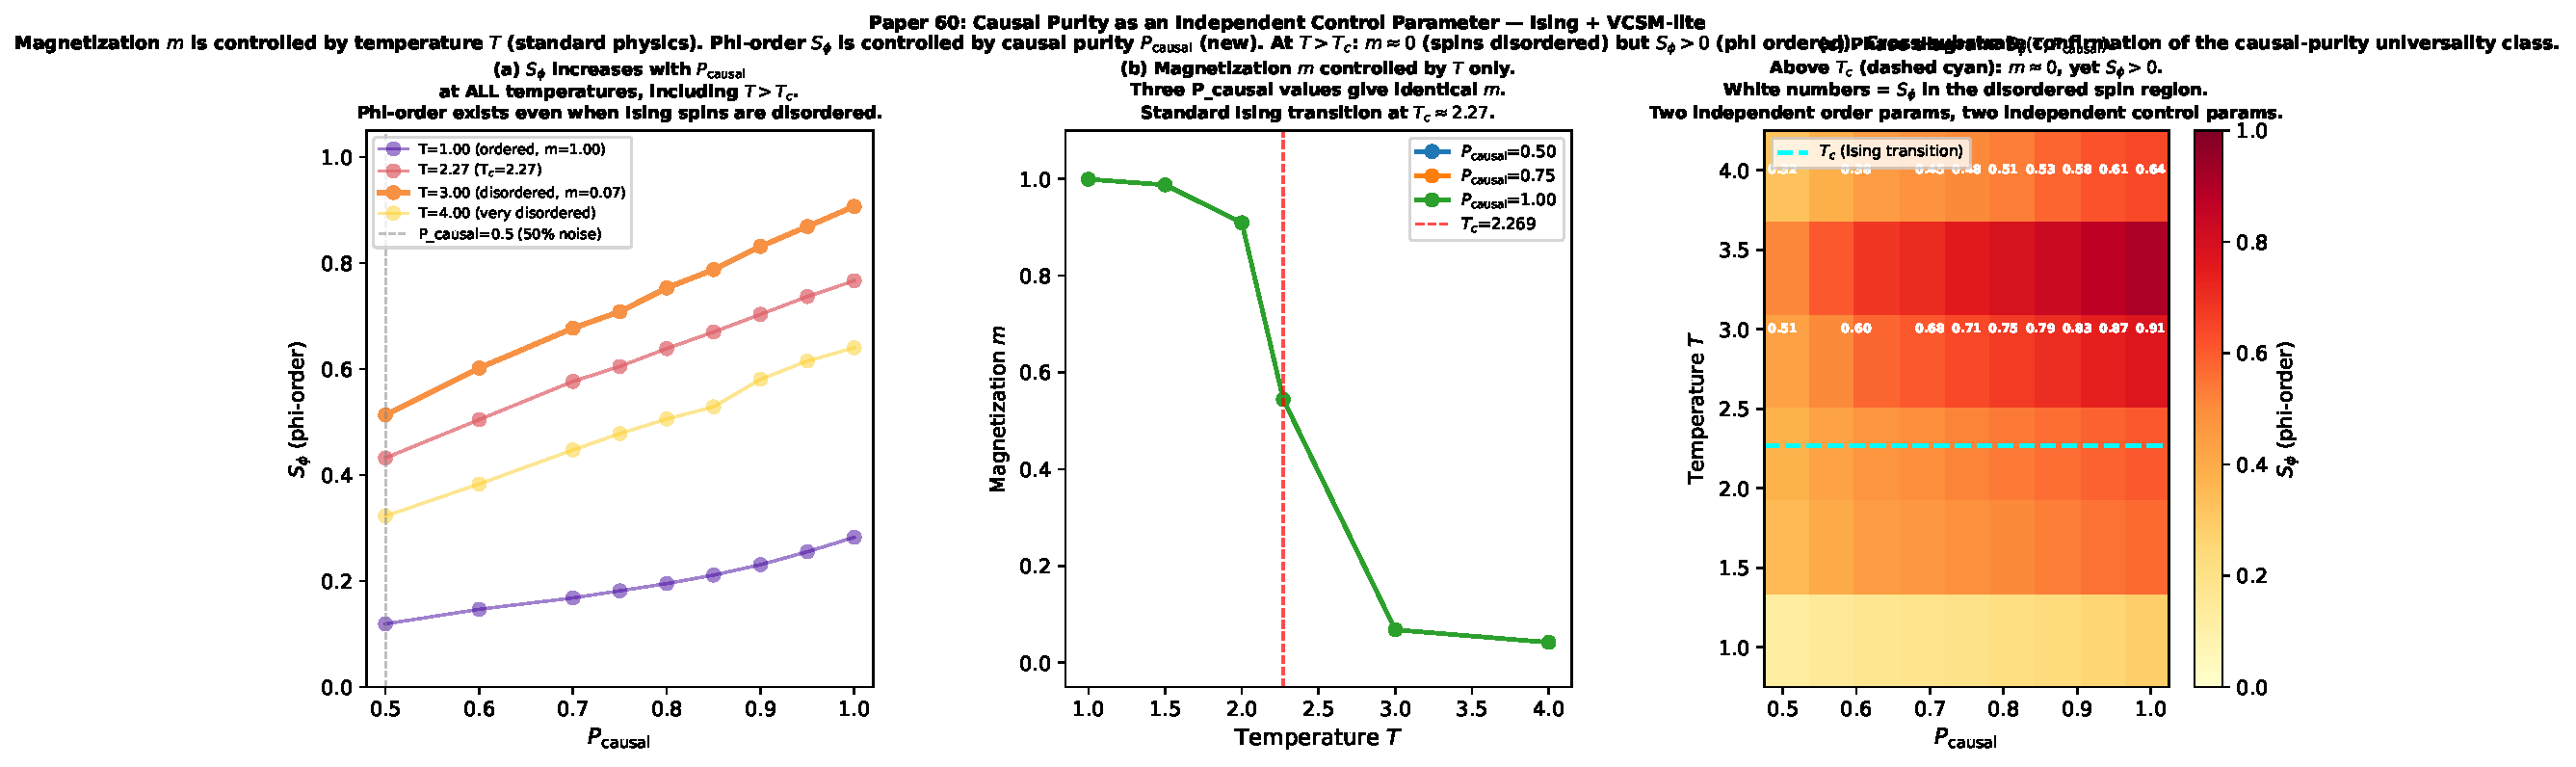
\includegraphics[width=\linewidth]{paper60_figure1.pdf}
  \caption{(a) $S_\phi$ vs $P_\mathrm{causal}$ at four temperatures.
    At $T=3.0$ (Ising disordered, $m=0.07$), $S_\phi$ increases
    from $0.51$ to $0.91$ with $P_\mathrm{causal}$ --- phi-order exists
    without spin order.
    (b) Magnetisation $m$ vs $T$ at three $P_\mathrm{causal}$ values:
    identical curves confirm $m$ is $P_\mathrm{causal}$-independent.
    (c) Phase diagram heatmap: $S_\phi(T, P_\mathrm{causal})$.
    Above the cyan dashed line ($T_c$): spins disordered but
    $S_\phi > 0$ and growing with $P_\mathrm{causal}$ (white annotations).
    Two independent phase structures, two independent control parameters.}
  \label{fig:main}
\end{figure}

\end{document}
